\documentclass[11pt, oneside]{article}   	% use "amsart" instead of "article" for AMSLaTeX format
\usepackage{geometry}                		% See geometry.pdf to learn the layout options. There are lots.
\geometry{letterpaper}                   		% ... or a4paper or a5paper or ... 
%\geometry{landscape}                		% Activate for for rotated page geometry
%\usepackage[parfill]{parskip}    		% Activate to begin paragraphs with an empty line rather than an indent
\usepackage{graphicx}				% Use pdf, png, jpg, or eps� with pdflatex; use eps in DVI mode
								% TeX will automatically convert eps --> pdf in pdflatex		
\usepackage{amssymb}
\usepackage{amsmath}
\usepackage{mathrsfs}
\usepackage{subcaption}

\newtheorem{definition}{Definition}[section]
\newtheorem{theorem}{Theorem}[section]
\newtheorem{conjecture}{Conjecture}[section]
\newtheorem{lemma}{Lemma}[section]
\newtheorem{conj}{Conjecture}[section]
\newtheorem{corollary}{Corollary}[section]
\newtheorem{remark}{Remark}[section]
\newtheorem{proposition}{Proposition}[section]
\newtheorem{assumptions}{Assumptions}[section]

\title{Computing spherical cap discrepancy.\\\small{DRAFT}}
\author{ }
%\date{}							% Activate to display a given date or no date

\begin{document}
\bibliographystyle{alpha}
\maketitle
\abstract{}

\subsection*{lit}

\cite{dobkin1993random}
\cite{dobkin1993computing}

\cite{dobkin1996computing}
\cite{brauchart2015distributing}
\cite{aistleitner2012point}
\cite{stolarsky1973sums}
\cite{brauchart2013simple}
\cite{beck1987irregularities}
\cite{gnewuch2009finding}
 \cite{doerr2005bounds}
 \cite{niederreiter1972discrepancy}
 \cite{matousek2009geometric}
 \cite{chazelle2000discrepancy}

\section*{Introduction}

The problem of computing discrepancy is known to be difficult as the dimension of the ambient space grows.  However, the problem of computing discrepancy in a fixed, low dimension is also if interest in integration theory, graphics and geometry.   In this paper, we present algorithms for computing the spherical cap discrepancy of point sets, discuss their implementation, and start a taxonomy of spherical point sets.

Originally, discrepancy was a number-theoretic function associated to a sequence of points $\{x_i\}$ in an interval.  The discrepancy measures the irregularity of the distribution of the sequence when truncated. 
\[
D_N(\{x_i\}) = \sup_{0 \le a < b \le 1} |\frac{\#( \{x_i\}_{i\le N)} \cap [a,b]}{N} - (b-a)|.
\]
A sequence is equidistributed if and only if the discrepancy is asymptotically zero.  There are several classical theorems in the area that give bounds on the rates of convergence.  See \cite{beck1987irregularities} for a comprehensive overview.  This notion can be generalized in many ways to other spaces, for example, by identifying the end points of the interval and including all connected subsets containing the point $0=1$.  This defines a discrepancy for a sequence of points on $\mathbb{S}^1$, the spherical cap discrepancy on the circle.  

In general, given a geometric sphere  $\mathbb{S}^{d}$ with radius 1 and normalized uniform measure $\sigma$ and an (open) spherical cap $C$ embedded in $\mathbb{R}^{d+1}$, the \emph{ local spherical cap discrepancy} of a set $X_N$ of $N$ distinct points in the $d$-sphere is given by
\[
\operatorname{D}_C[X_N] := |[\operatorname{Vol}(C) - \frac{1}{N}\# |X_N \cap C| ]|.
\]
This may be viewed as a normalized difference between the expected number of points in a cap of Vol($C$) and the number of points found in cap $C$
\[
\operatorname{D}_C[X_N] = \frac{1}{N}( \mathbb{E}[ \# |X_N \cap C|]- \#|X_N \cap C|) .
\]

When integrated over the space of caps of fixed size (equivalently, integrated over the sphere), this defines a variance
\[
\operatorname{Var}_C[X_N] = \int_{\mathbb{S}^{d}} \operatorname{D}_C^2 \,\mathrm{d} \sigma.
\]
There are several measurements of the quality of the point set based on this method.  
One is the spherical cap discrepancy, given as 
\[
\operatorname{D}(X_N) := \sup _{C\in \mathbb{S}^{d}\times [-1,1]}\operatorname{D}_C[X_N].
 \]
Another is the $\mathbb{L}^2$ discrepancy, given by
\[
\operatorname{D}_{\mathbb{L}^2}[X_N]:= \sqrt{\int_{-1}^{1} \operatorname{Var}_{C(t)}[X_N]\,\mathrm{d}t}
\]
where $C(t)$ is a cap defined by it's center $z$ and all points with inner product greater than $t$. Note:  the local discrepancy is symmetric through the boundary of the cap, so these integrals double count in some sense.   In the case of the $\mathbb{L}^2$ discrepancy, the integrand is the \emph{variance} of the point set for a fixed cap size.


\section{Algorithms}
\subsection{Naive}
--
\subsection{Pre-computation}
--
\subsection{Sweep-sorting}
\subsubsection{Topological sweeping}

Precomputing against low discrepancy sets can be worthwhile for min/mac based comparison algorithms, speed up minimal separation?

\section{remove or discuss ways of computing variance better?  is there a stolalrsky principle??}

We consider the variance of a point set in terms of spherical discrepancy....  The local discrepancy, (defined later) gives a discrete, finite collection of points, (resp. a measurable function)

Has expected value $$\int_{S^n} \frac{1}{N}\chi - \sigma$$ which has expected value 0

or, the expected number of points in a cap is exactly the area...   this can be seen geometrically?...  The volume of caps that contain any particular point is equal to the volume of the cap so decompose the integral into and the hight functions into a sum over volumes of caps contain particular points.... or this is just from the definition...

then the number variance is the same as the square of the discrepancy....


We consider the order of a uniformly random set of points and wish to do better.

\begin{remark}
There is a dependance on the choice of $\phi$.  Because the radius of the cap and the ambient sphere are not independent, the can be cancelation in the space of spherical harmonics for certain values.  Expanding with respect to $\phi$ that are in some way commensurate with the sphere leads to missing terms; the caps of that size cannot see certain symmetries.  For example, caps of radius $\pi/2$ will see point sets that a well distributed on a great circle as very regular, since almost all caps of that size will equally partition the set.  \emph{FIX This appears in the the expansion as missing all terms of a certain symmetry type....}\end{remark}


\section{Tables}

\subsection{Discrepancy: definitions and pictures}

\begin{figure}[htbp]
   \centering
   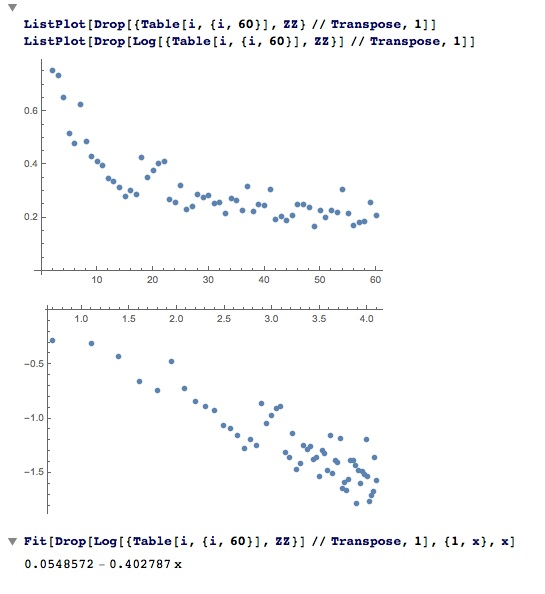
\includegraphics[scale=.4]{random1.jpg} % requires the graphicx package
   \caption{Discrepancy $\approx 0.0548572 - .0402787x$}
\end{figure}

\begin{figure}[htbp]
\begin{subfigure}{.5\textwidth}
   \centering
   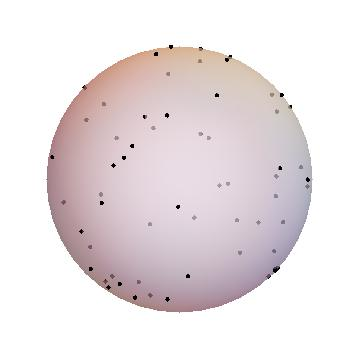
\includegraphics[scale=.4]{random60.jpg} % requires the graphicx package
   \caption{60 pseudorandom points}
\end{subfigure}
\begin{subfigure}{.5\textwidth}
   \centering
   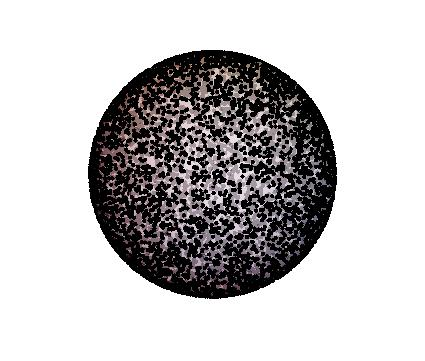
\includegraphics[scale=.4]{random2.jpg} % requires the graphicx package
   \caption{10000 pseudorandom points}
   \end{subfigure}
\end{figure}



\begin{figure}[htbp]
   \begin{subfigure}{.5\textwidth}
   \centering
   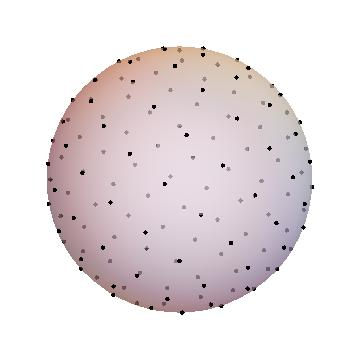
\includegraphics[scale=.4]{fib12front.jpg} % requires the graphicx package
   \caption{}
\end{subfigure}
\begin{subfigure}{.5\textwidth}
   \centering
   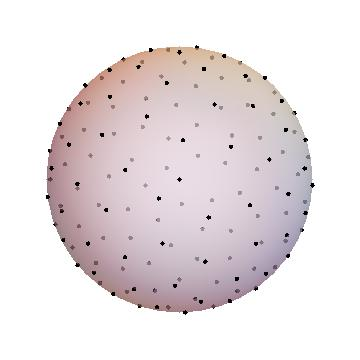
\includegraphics[scale=.4]{fib12top.jpg} % requires the graphicx package
   \caption{}
   \end{subfigure}
\end{figure}

\begin{figure}[htbp]
   \centering
   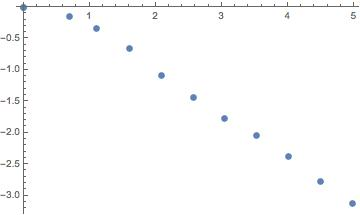
\includegraphics[scale=.4]{linearfib.jpg} % requires the graphicx package
   \caption{Discrepancy $\approx 0.474954 - 0.725491 x$}
\end{figure}


\begin{figure}[htbp]
\begin{subfigure}{.4\textwidth}
   \centering
   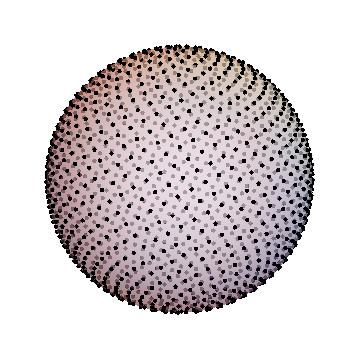
\includegraphics[scale=.4]{fib17front.jpg} % requires the graphicx package
   \caption{}
\end{subfigure}
\begin{subfigure}{.4\textwidth}
   \centering
   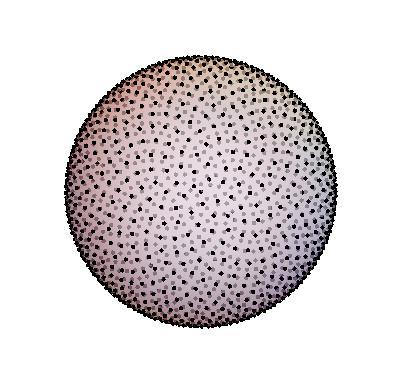
\includegraphics[scale=.4]{fib17top.jpg} % requires the graphicx package
   \caption{}
   \end{subfigure}
\end{figure}

\begin{figure}[htbp]
   \centering
   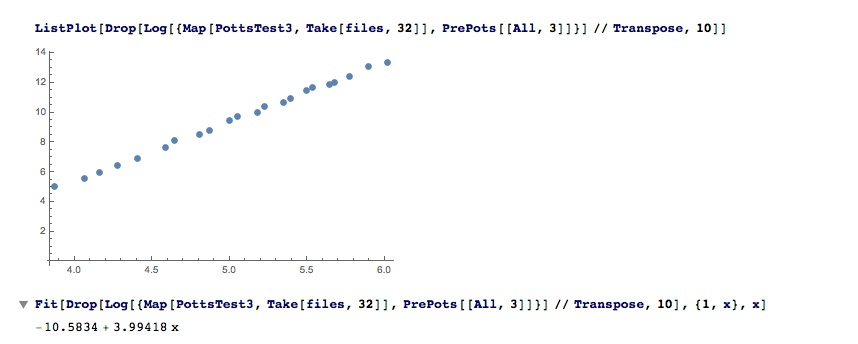
\includegraphics[scale=.4]{runtime.jpeg} % requires the graphicx package
   \caption{Runtime $\approx -10.5834 - 3.99418x$}
\end{figure}

\begin{figure}[htbp]
   \centering
   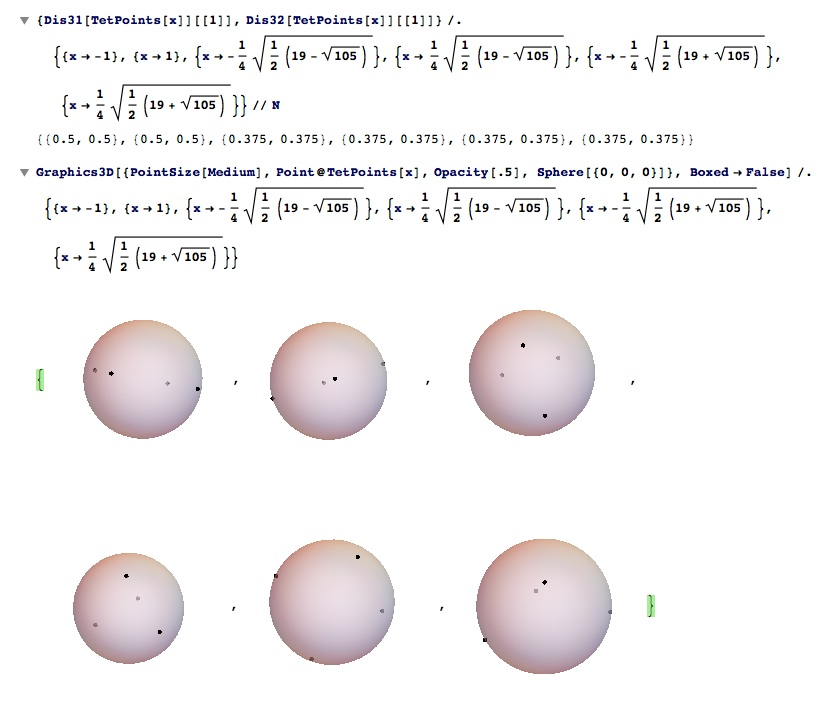
\includegraphics[scale=.3]{optsimp.jpeg} % requires the graphicx package
\end{figure}

 \begin{figure}[htbp]
      \centering
      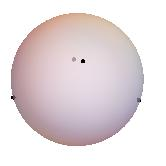
\includegraphics[scale=1]{tetpoints.jpg} % requires the graphicx package
\caption{minimal discrepancy configuration of 4 points}
   \end{figure}


      \begin{figure}[htbp]
      \centering
      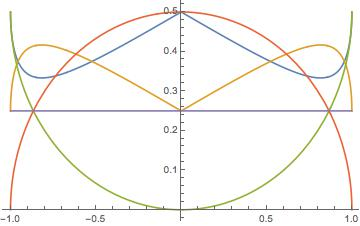
\includegraphics[scale=.9]{discrepancygraph.jpg} % requires the graphicx package
\caption {discrepancies in t-parameter for 4 points}
   \end{figure}
   
   Uniqueness of the minimal discrepancy configuration
   As expected, this is not universal



\subsection{Reproducing Kernel}

The arguments of \cite[\S 2]{brauchart2013simple} seem to pass through by deleting the outer integral integration.  One obtains a kernel $K : \mathbb{S}^d \times \mathbb{S}^d \rightarrow \mathbb{R}$
\[
K_{\mathscr{C}(t)}(x,y) = \int_{\mathbb{S}^d} \chi_{C(z,t)}(x)\chi_{C(z,t)}(y) \,\mathrm{d}\sigma
\]
This is symmetric and positive definite.  In fact, it is the area of the intersection of spherical caps of radius $t$ centered at $x$ and $y.$  By Moore-Aranszajn, there is a unique Hilbert space of functions on $S^d$ for which this is a reproducing kernel. This includes functions with integral representation 
\[
f(x)=  \int_{\mathbb{S}^d}  g(z) \chi_{C(z,t)}(x)(y) \,\mathrm{d}\sigma
\]
where $g$ is an $\mathbb{L}^2(\mathbb{S}^d)$ function from $\mathbb{S}^d \rightarrow \mathbb{C}$.


Asymptotics, the caps go to zero, with a normalization 
\[
f^*(x)=  \frac{1}{Vol[C(t)]}\int_{\mathbb{S}^d}  g(z) \chi_{C(z,t)}(x)(y) \,\mathrm{d}\sigma
\]
then differentiable? $f(x) = g(x)$ $a.e.$?  

By construction, nontrivial functions of this type certainly exist (at least for some values of $t$) and satisfy a mean value property/averaging property the value $f(x)$ is the volume weighted average value of the function on the cap centered at $x.$  So for small caps, the function space is probably large(topological issues?  images of harmonic functions glued on the boundary?  since these are really classes of functions, can we get away with more?)  

\[
f(x) = Vol(C) \cdot MV(g|_C)
\]

In the case of the whole sphere, this certainly this must be a constant function (and it is indeed correctly weighted)

More details on what are these function spaces???

Also, not that this kernel $K_{C,t}(x,y)$ is given by the intersection volume of two spherical caps of radius t centered at x and y respective, so it has some closed form in terms of volumes, which might need to restrict to the case where caps are of volume less than $1$.

Note: does this give a distributional version of the weighted discrepancy.

This kernel is a function of the inner product and for $\mathbb{S}^2$ is given by

This kernel does not have an elegant expression in terms of spherical geometry, but it can be expressed in a piecewise fashion.  

This kernel is analogous to the window device used in hyperuniformity and the "structure factor?" 

\[
K(x\cdot y) = \left\{
     \begin{array}{lr}
       0 &  \textrm{ for }  x\cdot y \ge t\\
       trianfds &   \textrm{ for }  x \cdot y \le t
     \end{array}
   \right.
\]


Zweieck (lune/digon) discrepancy

\subsection{Expansion of the Kernel}
...
Integrate against the spherical harmonics w.r.t. measure for the correct Hilbert space?   this is a nested collection of Hilbert spaces, how does the reproducing kernel behave?  it should some kind of sequence or chain or "semi norm type object."


Consider the case of where the cap is a hemisphere.  Then the area of intersection is given by the angle between two points.  This is equivalent to the $\mathbb{S}^1$ case, where 
\[
K_\phi(x\cdot y) = \max[\frac{\phi - \arccos(x\cdot y)}{2\pi},0]
\]
which becomes simply
\[
K(x\cdot y) = \frac{\pi - \arccos(x\cdot y)}{2\pi}
\]
Note that in this case, the kernel is 




at the other end, there is an infinitesimal ...


Kernel for $S^2$  

$$
0 \textrm{ or } 2 \left(-2 \tan ^{-1}\left(\sec (\rho ) \cos \left(\frac{1}{4} \left(2 \rho +\cos
   ^{-1}(t)\right)\right) \sec \left(\frac{\rho }{2}-\frac{1}{4} \cos ^{-1}(t)\right)
   \tan \left(\frac{1}{4} \left(2 \sin ^{-1}\left(\csc (\rho ) \sin \left(\frac{1}{2}
   \cos ^{-1}(t)\right)\right)+\pi \right)\right)\right)
   +(2-4 \cos (\rho )) \cot
   ^{-1}\left(\cos \left(\frac{1}{4} \left(2 \rho +\cos ^{-1}(t)\right)\right) \sec
   \left(\frac{\rho }{2}-\frac{1}{4} \cos ^{-1}(t)\right) \tan \left(\frac{1}{4} \left(2
   \sin ^{-1}\left(\csc (\rho ) \sin \left(\frac{1}{2} \cos ^{-1}(t)\right)\right)+\pi
   \right)\right)\right)+\pi \right)
$$

OR??

$$
\frac{2 \left(1-\cos \left(\frac{\phi }{2}\right)\right) \cos ^{-1}\left(\cot \left(\frac{\phi }{2}\right) \tan \left(\frac{1}{2} \cos
   ^{-1}(t)\right)\right)-2 \cos ^{-1}\left(\cot \left(\frac{\phi }{2}\right) \tan \left(\frac{1}{2} \cos ^{-1}(t)\right)\right)-2 \sin
   ^{-1}\left(\csc \left(\frac{\phi }{2}\right) \sin \left(\frac{1}{2} \cos ^{-1}(t)\right)\right)+\pi }{2 \pi }
$$

\subsection{Worst Case Error}


\subsection{Example}

Consider the case of where the cap is a hemisphere.  Then the area of intersection is given exactly by the angle between two points.  



\section{Geometry}
\subsection{Simplices}
Discrepancy for a top dimensional simplex. Duality 

The minimal discrepancy of four points on $\mathbb{S}^2$ is ...

By symmetry, if the duality is strong, the discrepancy between caps is a stationary point as points on the boundary pass between each other...

\[
|Vol(C_{min}) -\frac{1}{4}| = |1-Vol(C_{min})|
\]
and therefore there is a lower bound on the minimal discrepancy of $3/8$.  There are examples of point sets that achieve this 3-minimal discrepancy given by "flattened" and "stretched" regular simplices:

\[  
\begin{array}{lr}
(0, \frac{1}{4} \sqrt{\frac{1}{2} (19 + \sqrt{105})}, \sqrt{1 + \frac{1}{32} (-19 - \sqrt{105})}),\\
(0, -\frac{1}{4} \sqrt{\frac{1}{2} (19 + \sqrt{105})},\sqrt{1 + \frac{1}{32} (-19 - \sqrt{105})}),\\
(\frac{1}{4} \sqrt{\frac{1}{2} (19 + \sqrt{105})},0, -\sqrt{1 + \frac{1}{32} (-19 - \sqrt{105})}),\\
(-\frac{1}{4} \sqrt{\frac{1}{2} (19 + \sqrt{105})}, 0, -\sqrt{1 + \frac{1}{32} (-19 - \sqrt{105})})
\end{array}
\]  
 
 and
 
\[  \begin{array}{lr}
(0, \frac{1}{4} \sqrt{\frac{1}{2} (19 - \sqrt{105})}, \sqrt{1 + \frac{1}{32} (-19 + \sqrt{105})}),\\
(0, -\frac{1}{4} \sqrt{\frac{1}{2} (19 - \sqrt{105})},\sqrt{1 + \frac{1}{32} (-19 + \sqrt{105})}),\\
(\frac{1}{4} \sqrt{\frac{1}{2} (19 - \sqrt{105})},0, -\sqrt{1 + \frac{1}{32} (-19 + \sqrt{105})}),\\
(-\frac{1}{4} \sqrt{\frac{1}{2} (19 - \sqrt{105})}, 0, -\sqrt{1 + \frac{1}{32} (-19 + \sqrt{105})}).
\end{array}
\]  

With respect to the 2-minimal discrepancy, we see that only one of these is of minimal discrepancy
 
 
 
 
 
For $d+2$ points $\mathbb{S}^d$, a similar argument gives an asymptotic lower bound on discrepancy growing to 1/2 as the dimension grows.  This is expected as a consequence of the concentration of measure for spheres, that is that measure concentrates about the equator (in fact about all great circles), in that the volume of a neighborhood of any great circle is large.  This phenomenon is also seen in the concentration of measure towards the boundary of a solid ball in high dimensions.





\section{scratch}
weighted $\mathbb{L}^2$-discrepancy gives a way to approximate...

define

the cap discrepancy

the variance

Then the l2 discrepancy becomes

the sup discrepancy becomes

the l2 discrepancy can be partitioned in other ways

i.e. over fixed sigma volume

over fixed delta volume regions

over fixed indexed delta volume regions

over different integrands

annealing problems

The kernel associated to the variance.

----

approximations

weighted discrepancy





minimization of discrepancy

----

asymptotics

the rescaling rates
the normalization
asymptotics in dimensions

for regular simplex dot product is -1/n

Johnson Lindestrauss  extremeal combinatorics

http://mathoverflow.net/questions/24864/almost-orthogonal-vectors

note::: almost orthogonal vector sets grow quickly...

\section{Computing spherical cap discrepancy}

\subsection{bounds for the spherical cap discrepancy}

\subsection{computing the cap discrepancy}

Conjecture:  An $\mathbb{L}^p$ discrepancy for $\mathbb{L}^\infty$ results (Brauchart)

References[\cite{gnewuch2009finding} \cite{doerr2005bounds},\cite{niederreiter1972discrepancy}]

The \emph{star discrepancy} of a set $X$ of $N$ distinct points in the $d$-cube is given by
\[
...
\]
In the case of the star discrepancy an algorithm was described in \cite{niederreiter1972discrepancy} that exactly computes the star discrepancy as follows
...

for spherical cap discrepancy

....

\subsection{naive algorithm}
This is of the order $O(dN^{d+k})$ as it may be viewed as choosing d-tuples of coordinates from the array of coordinates given by $X \cup \{0\} \cup \{1\} $

Similarly, the spherical cap discrepancy of can be exactly computed by considering all hyperplanes defined by $d$ points on $\mathbb{S}^{d-1}$ as well as the special hyperplanes defined by lower dimension collections that "capture" the intersection caps....

In the case of $\mathbb{S}^2$...

It is clear that the maximum discrepancy occurs can be restricted to the consideration of such caps with the appropriate assignment of points, which can be assigned checking each point against a normal. 

describe geometric flow of the circles.  When the boundary of a cap does not contain a point in X, it is either balanced it is clear that  the area can be decreased (or increased) by flowing toward a pole (or if a geodesic, it partitions the set in such a way that discrepancy can also be increased by flowing towards on pole or the other) without changing the number of points contained. Therefore it must not be a maximizer for the discrepancy. 

As soon as the boundary captures a point, it may be anchored there and remain a region of the space of spherical caps where the discrepancy function is continuous.  By similar geometric arguments as above, 

the boundary may be flowed without passing points to (a) contract around a single point, to become trapped around two points that are diametrically opposite (possibly the cap still contains more points), or become trapped on three points.  Since 3 points (and in general $d$ points) define a plane (and thus a cap), it is clear that one need only consider the subsets of X with cardinality less than or equal to 3, and the possible assignments of points to each cap (points on the boundary may be inside or outside.)

 (( It is clear the the maximum discrepancy occurs on the bouquets of circles emanating from the point set X.  )
symmetry of the discrepancy is this case (as with in the star case???) allows the free swapping across the boundary of the various caps)

even the brute is polynomial in the number of points..... as one has uniformly bounded subset problem where one compares every point in X to every subset of cardinality less than or equal to $d$





\subsection{Implementation/technical report}
A naive numerical implementation of the brute force algorithm Mathematica allowed for approximating the discrepancy of the $Fib[12]=144$ points in $< 10000s$.  

Parallel
NOT OPTIMIZED IN MATHEMATICA
reimplemented in python, parallel package on cpus
will move to gpus
Run it in C?
 
Uses NO symmetry/special properties.sorting to reduce subsets problem considered.
possibly sorting count give a pretty big decrease in time/memory, (right now, everything is called 4 times...)

It is unclear how Mathematica implements various functions internally, for example, using a DO loop (Olekander, Soren, Theran) does not seem to give a significant improvement. 

By using matrix multiplication, it is possible to improve the run time by a factor of about 100 (private correspondence with Loiuis Theran) and is possible to easily parallelize, but a high memory cost.



There is an error associated to the points on the boundary of the caps, that should be eliminated. or analyzed

A log plot indicates that the algorithm is approximately of order $O(n^4)$.

Using the original implementation, the spherical cap discrepancy of the Potts list of Quadrature points was computed to...

Spherical Fibonacci lattice points were computed to...

Pseudo-Random points were computed to...

Lots of pictures...



\subsection{bounds for the $\mathbb{L}^2$ discrepancy}

\cite{aistleitner2012point}

\subsection{computing the $\mathbb{L}^2$ discrepancy}

\cite{stolarsky1973sums}
\cite{brauchart2013simple}

Stollarsky invariance formula

weighted version

piecewise discrepancy of sets

trivial lower bounds
trivial upper bounds

the discrepancy map

minimal energy

worst case error

convolution and integrators

other functions

\subsection{bounds for the variance}

\subsection{computing the variance}

\subsection{minimization of discrepancy}


sketch, consider the minimum if it satisfies certain properties, allows one to pass support points across the boundary (duality property...) in s2, caps are supported by 3 pts (or fewer, need to make stronger...)
\[
Dmin = |Vcap - 1/4 | = |1-Vcap|
\]

and therefore $V = 5/8$ and $D = 3/8$

generally, something like 
\[
Dmin = |1 - (1-1/(2d+2))| \rightarrow 0
\]
might hold if the duality principle holds...

AND it might be easy to find.  of course, this is for normalized measure on the sphere, and the surface area goes to zero as well (at the same rate??), so it is probably not so useful for applications.  Unless the normalized measure is what is needed?





QUESTION!  WHAT IS THE DISCREPANCY OF THE REGULAR SIMPLEX IN HIGH DIMENSIONS?

IS A MINIMAL DISCREPANCY SET OF SIZE D+1 A REALLY GOOD SET?
Is there a projection to a lower sphere that is good?  a projection to a random great circle?  A best great cicle?
 probably not, since the surface area shrinks and so the normalization means that the the radius of such a ball grows and the euclidean separation must grow too.

\section{Hyperuniformity}

To investigate hyperuniformity in the sense of Torquato and Stillinger [],  it is necessary to consider the variance of a point set with respect to a window. In the case of point process, it is possible to pass to the thermodynamic limit, freeing one to consider only the size of the window.

On a compact space it is less readily apparent what the analogous process should be.

  Consider the sphere. One can consider a sequence of points $\{x_n\}_{n\rightarrow \infty}$, or even a sequence of point sets $\{X_n\}_{n\rightarrow \infty}$.  The latter case will be the desired case, as it contains contains the sequence of points as a subset and also contains a richer collection of examples.

Should we consider the base space or the configuration space as a tower of point sets?  

In the case of a compact set, the problem is that the we cannot pass to the limit, so there is no was to have infinite wavelength fluctuations, and obviously, the variance is bounded etc...  define hyper uniformity is several ways in terms of structure factor  

there is the problem of taking the Fourier transform of the point process?  there are ways to do this in terms of the representation theory of the space (of functions) we are studying.  

First, define a spherical cap as before.

For a fixed point set $X_n$ and a fixed cap size $t$, the expected value of a (normalized point set) is simply the area of the cap.
Then the variance can be viewed as a that of a weighted discrete random variable, and is given by the $L^2$ discrepancy for a fixed cap size.

This then has a kernel representation as ...

From [], it is possible to describe this a weighted L2 function given by a delta sequence of weights at a chosen value in $[-1,1]$

maybe, maybe not, the asymptotics look bad w.r.t. that paper...

\subsection{asymptotics}

point processes...  thermodynamic limit

As the number of points grows, ...

One definition of a hyper uniform process is that the number variance grows like the boundary.  For a discrete collection of points with fixed density, ...


in the compact setting, hyperuniformity is a question about the rate of rescaling at which the variance is stabilized.

That is, given a sequence of point sets, how does the variance behave?

sequences of points are more in keeping with the idea of a point process?


Clearly, pathological examples can be constructed when considering sequences of point sets, but it also allows for the consideration of sequences of minimizers that are not chains in the order theoretic sense.

concrete approach before a measure theoretic/probability approach


\section{blichfeldt gauges?}

\section{Riemann-Stiljes?}

...

Symmetry
Expectations
Large regions of high discrepancy
Sharpening inequalities

the equal area stuff

\section{multiple read heads and robustness}
The competitive ratio:  is it applicable to this area?

best algorithm for time optimization of a multiple read head system on a homogeneous space.  

The minimal discrepancy configuration moves together, it is in some sense maximally robust.  Note that the maximal separation configuration is NOT the most robust in the following sense.  This gives the best area concentration.  the most heads nearby...??? is that right, is this optimal in that sense???  There are the correct number inside each one, they cover well, have a good response time????  and a good support time...  

there are the correct number of points per area....???

this is not response time, this is coverage...


\section{Monge?}

\section{combinatorial optimization?}

1 partitioning

the proof of the optimality of configuration x for the 

sup discrepancy

problems with well-defined-ness of sup discrepancy

filtration of sup discrepancy

the optimality of the simplex for the variance

\bibliography{discrepancy}
\end{document}  